
\chapter{Arquitetura de Software}
\label{sec-arquitetura}
\vspace{-1cm}

A Figura~\ref{figura-arquitetura} mostra a arquitetura do sistema \emph{\imprimirtitulo}. Ela é baseada em uma combinação dos estilos arquitetônicos Camadas e Partições.

\begin{figure}[h]
	\centering
	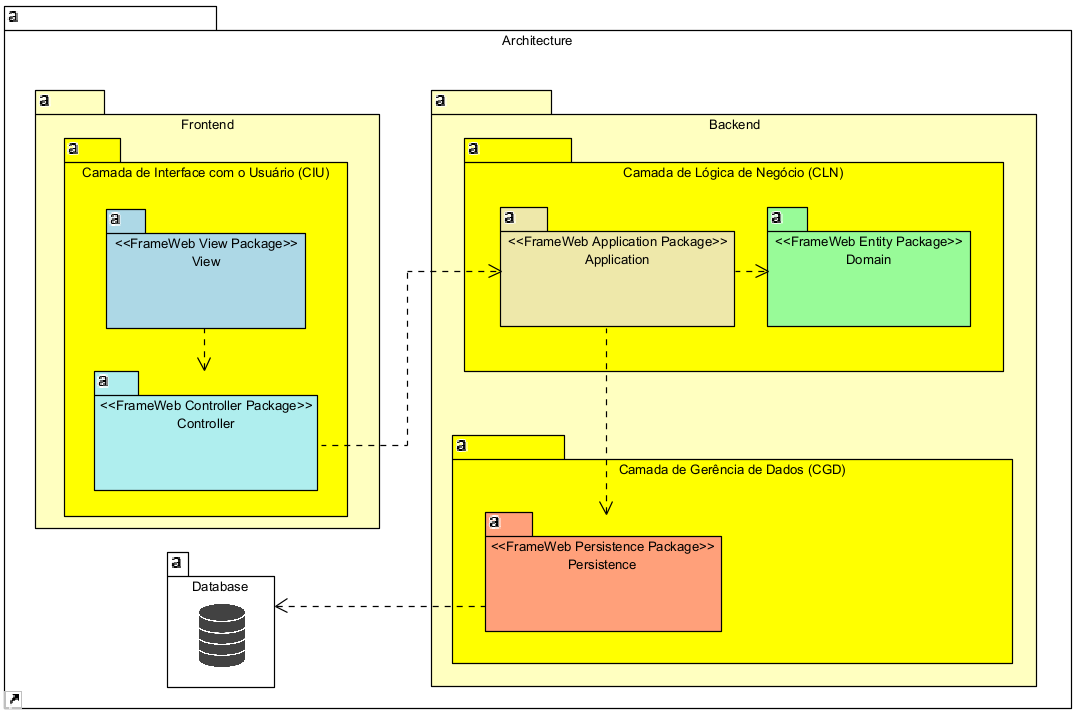
\includegraphics[width=0.8\textwidth]{figuras/architecture_novo.png}
	\caption{Arquitetura de Software.}
	\label{figura-arquitetura}
\end{figure}

A arquitetura do sistema é estruturada em três camadas principais, cada uma com responsabilidades distintas e bem definidas, conforme ilustrado na Figura ~\ref{figura-arquitetura}.

\section{Camada de Interface com o Usuário (CIU)}

Localizada no \textbf{Frontend}, essa camada é responsável pela interação com os usuários, exibindo dados e capturando ações externas. Ela adota o padrão \textbf{MVCS (Model-View-Controller-Service)} e está dividida em dois pacotes principais:

\begin{itemize}
	\item \textbf{View (\texttt{<<FrameWeb View Package>>})}: Contém os elementos da camada de apresentação, como páginas web, folhas de estilo, imagens e scripts do lado cliente.
	\item \textbf{Controller (\texttt{<<FrameWeb Controller Package>>})}: Coordena a interação entre a visão e os serviços da aplicação localizados na camada de lógica de negócio (CLN). A dependência entre os componentes é unidirecional: a \textit{view} depende do \textit{controller}, e este depende da lógica de aplicação.
\end{itemize}

\section{Camada de Lógica de Negócio (CLN)}

Localizada no \textbf{Backend}, essa camada implementa as regras de negócio do sistema. Ela segue o padrão \textbf{Camada de Serviço}, conforme definido por Fowler (2002), e é composta por dois pacotes:

\begin{itemize}
	\item \textbf{Application (\texttt{<<FrameWeb Application Package>>})}: Contém as classes responsáveis pela orquestração das funcionalidades do sistema, utilizando objetos de domínio e interagindo com a camada de persistência.
	\item \textbf{Domain (\texttt{<<FrameWeb Entity Package>>})}: Reúne as classes que representam os elementos centrais do domínio do problema. Tais entidades são manipuladas pela \textit{application} para a implementação das regras de negócio.
\end{itemize}

\section{Camada de Gerência de Dados (CGD)}

Também localizada no \textbf{Backend}, essa camada é responsável pela persistência dos dados e segue o padrão \textbf{Data Access Object (DAO)}. Contém o seguinte pacote:

\begin{itemize}
	\item \textbf{Persistence (\texttt{<<FrameWeb Persistence Package>>})}: Inclui as classes responsáveis pelas operações de acesso a dados, realizando mapeamento objeto-relacional (ORM) para persistir as entidades do domínio no banco de dados relacional.
\end{itemize}

\section{Integração entre as Camadas}

\begin{itemize}
	\item A \textbf{View} se comunica com o \textbf{Controller}.
	\item O \textbf{Controller} interage com a camada \textbf{Application}.
	\item A \textbf{Application} manipula entidades do \textbf{Domain} e utiliza a camada \textbf{Persistence} para realizar a persistência dos dados.
	\item A \textbf{Persistence} acessa diretamente o \textbf{banco de dados relacional}.
\end{itemize}

%\vitor{Substituir a Figura~\ref{figura-arquitetura} pelo diagrama UML da arquitetura do seu projeto e descrevê-la no texto. Caso use alguma arquitetura clássica, incluir referência bibliográfica com BibTeX (ex.:~\cite{fowler:book02}).}
